%% Auto-generated by scripts/generate_figures.py
\begin{figure}[htbp]
\centering
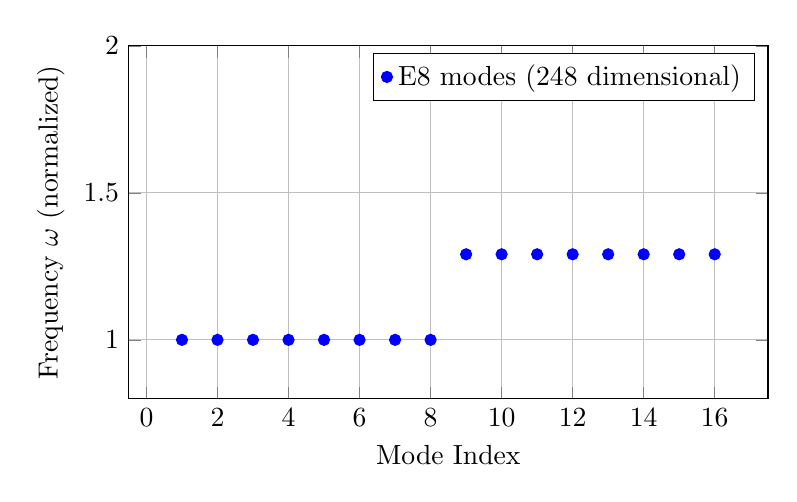
\begin{tikzpicture}
  \begin{axis}[
    width=0.8\textwidth,
    height=0.5\textwidth,
    xlabel={Mode Index},
    ylabel={Frequency $\omega$ (normalized)},
    grid=major,
    ymin=0.8,
    ymax=2.0
  ]
    \addplot[only marks, mark=*, blue] coordinates {
      (1.0000, 1.000000e+00)
      (2.0000, 1.000000e+00)
      (3.0000, 1.000000e+00)
      (4.0000, 1.000000e+00)
      (5.0000, 1.000000e+00)
      (6.0000, 1.000000e+00)
      (7.0000, 1.000000e+00)
      (8.0000, 1.000000e+00)
      (9.0000, 1.290994e+00)
      (10.0000, 1.290994e+00)
      (11.0000, 1.290994e+00)
      (12.0000, 1.290994e+00)
      (13.0000, 1.290994e+00)
      (14.0000, 1.290994e+00)
      (15.0000, 1.290994e+00)
      (16.0000, 1.290994e+00)
    };
    \addlegendentry{E8 modes (248 dimensional)}
  \end{axis}
\end{tikzpicture}
\caption{E$_8$ vibrational mode spectrum grouped by root orbit structure.}
\label{fig:e8-spectrum}
\end{figure}
